\documentclass[journal]{IEEEtran}
\usepackage[a5paper, margin=10mm, onecolumn]{geometry}
%\usepackage{lmodern} % Ensure lmodern is loaded for pdflatex
\usepackage{tfrupee} % Include tfrupee package

\setlength{\headheight}{1cm} % Set the height of the header box
\setlength{\headsep}{0mm}     % Set the distance between the header box and the top of the text

\usepackage{gvv-book}
\usepackage{gvv}
\usepackage{cite}
\usepackage{amsmath,amssymb,amsfonts,amsthm}
\usepackage{algorithmic}
\usepackage{graphicx}
\usepackage{textcomp}
\usepackage{xcolor}
\usepackage{txfonts}
\usepackage{listings}
\usepackage{enumitem}
\usepackage{mathtools}
\usepackage{gensymb}
\usepackage{comment}
\usepackage[breaklinks=true]{hyperref}
\usepackage{tkz-euclide} 
\usepackage{listings}
% \usepackage{gvv}                                        
\def\inputGnumericTable{}                                 
\usepackage[latin1]{inputenc}                                
\usepackage{color}                                            
\usepackage{array}                                            
\usepackage{longtable}                                       
\usepackage{calc}                                             
\usepackage{multirow}                                         
\usepackage{hhline}                                           
\usepackage{ifthen}                                           
\usepackage{lscape}
\begin{document}

\bibliographystyle{IEEEtran}
\vspace{3cm}

\title{11.16.3.2}
\author{EE24BTECH11001 - Aditya Tripathy}
 \maketitle
% \newpage
% \bigskip
{\let\newpage\relax\maketitle}

\renewcommand{\thefigure}{\theenumi}
\renewcommand{\thetable}{\theenumi}
\setlength{\intextsep}{10pt} % Space between text and floats


\numberwithin{equation}{enumi}
\numberwithin{figure}{enumi}
\renewcommand{\thetable}{\theenumi}


\textbf{Question}:\\
A coin is tossed twice, what is the probability that atleast one tail occurs?
\\
\textbf{Solution: }\\
The sample space is 
\begin{align}
  \Omega = \cbrak{HH, HT, TH, TT}
\end{align}
Assuming equally likely outcomes, 
\begin{align}
  \Pr\brak{\omega \in \Omega} = \frac{1}{4}
\end{align}
Define a discrete random variable X = number of tails in the sequence.
\newline
Probability Mass Function $\Pr_{X}\brak{x}$ is given by:
\begin{align}
  \Pr_{X}\brak{x} = \begin{cases}
\frac{1}{4} & x = 0\\
    \frac{1}{2} & x = 1\\
    \frac{1}{4} & x = 2\\
\end{cases}
\end{align}
The CDF (Cumulative Distribution Function) is given by:
\begin{align}
  F_{X}\brak{x} = \Pr_X\brak{X \le x} = \begin{cases}
    0 & x < 0\\
    \frac{1}{4} & 0 \le x < 1\\
    \frac{3}{4} & 1 \le x < 2\\
    1 & x >=2
  \end{cases}
\end{align}
\begin{align}
  \Pr\brak{X \ge 1} &= 1 - \Pr\brak{X < 1}\\
  &= 1 - \frac{1}{4} = \frac{3}{4}
\end{align}
Simulation:
\newline
To run a simulation we need to generate random numbers with uniform probability, which is done
as shown below(Algorithm taken from OpenSSL's random\_uniform.c):
\begin{enumerate}
  \item \text{Generate 32 bits of entropy using /dev/urandom.}
  \item Treat this as a fixed point number in the range [0, 1)
  \item Scale this to desired range using fixed point multiplication and treat as 64bit number(upper 32 bits integer and rest as fractional part)
  \item Return the integer part of the fixed point numbers
\end{enumerate}
The following shows how the relative frequency reaches true probability with increasing number of trials of the event.
\begin{figure}[h!]
   \centering
   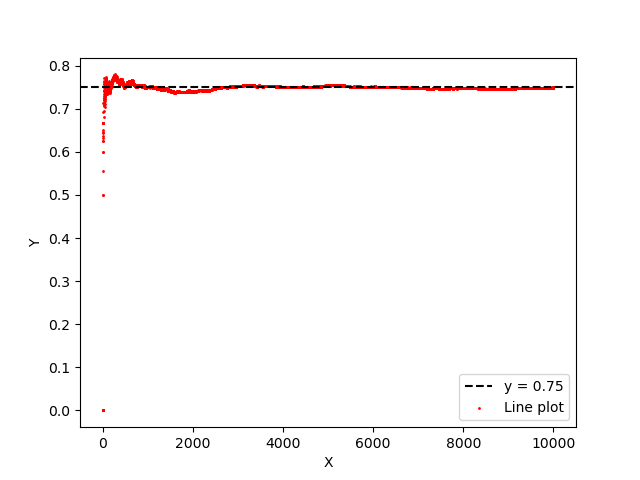
\includegraphics[width=0.7\columnwidth]{figs/fig.png}
    \caption{Relative Frequency tends to True Probability}
\end{figure}
\begin{figure}[h!]
   \centering
   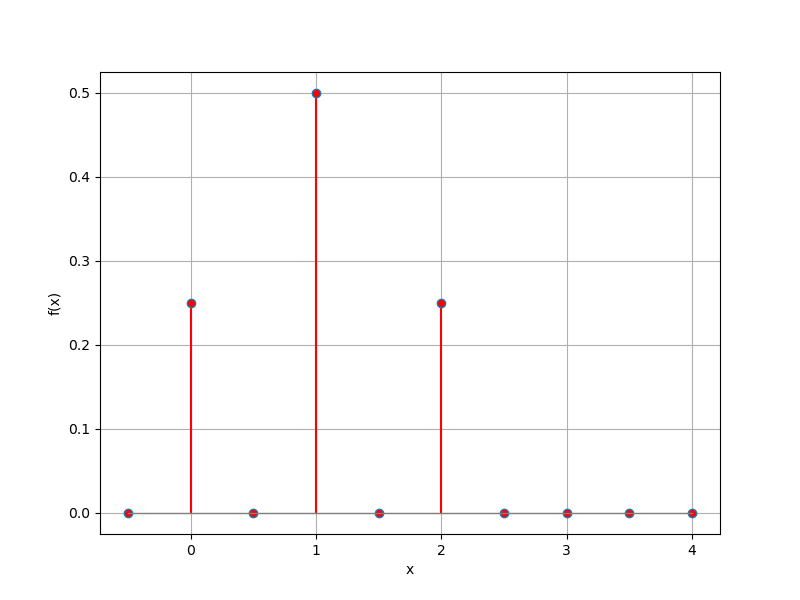
\includegraphics[width=0.7\columnwidth]{figs/fig1.png}
    \caption{Probability Mass Function}
\end{figure}
\begin{figure}[h!]
   \centering
   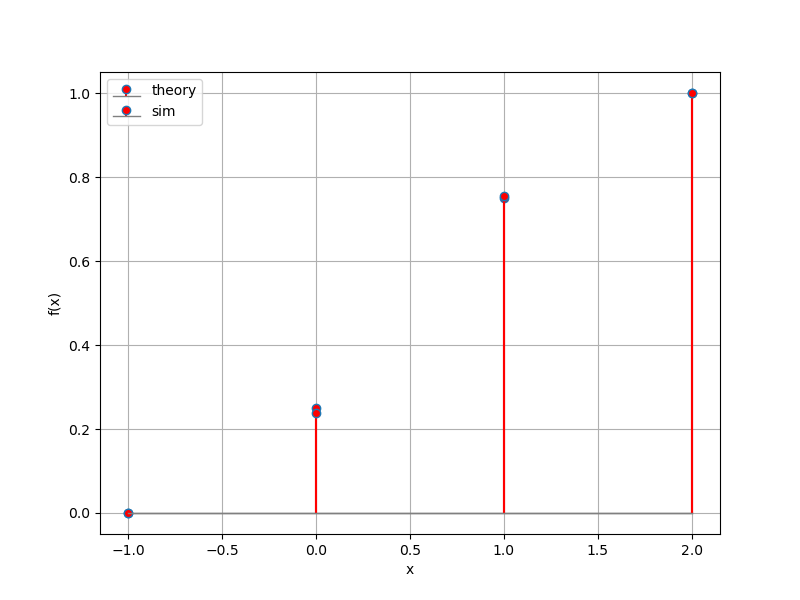
\includegraphics[width=0.7\columnwidth]{figs/fig2.png}
    \caption{Cumulative Distribution Function}
\end{figure}
\end{document}

